\documentclass[12pt,preprint]{aastex}

% has to be before amssymb it seems
\usepackage{color,hyperref}
\definecolor{linkcolor}{rgb}{0,0,0.5}
\hypersetup{colorlinks=true,linkcolor=linkcolor,citecolor=linkcolor,
            filecolor=linkcolor,urlcolor=linkcolor}

\usepackage{url}
\usepackage{algorithmic,algorithm}
\usepackage{amssymb,amsmath}

\usepackage{listings}
\definecolor{lbcolor}{rgb}{0.9,0.9,0.9}
\lstset{language=Python,
        basicstyle=\footnotesize\ttfamily,
        showspaces=false,
        showstringspaces=false,
        tabsize=2,
        breaklines=false,
        breakatwhitespace=true,
        identifierstyle=\ttfamily,
        keywordstyle=\bfseries\color[rgb]{0.133,0.545,0.133},
        commentstyle=\color[rgb]{0.133,0.545,0.133},
        stringstyle=\color[rgb]{0.627,0.126,0.941},
    }

\newcommand{\project}[1]{{\sffamily #1}}
\newcommand{\Python}{\project{Python}}
\newcommand{\numpy}{\project{numpy}}
\newcommand{\bart}{\project{Bart}}
\newcommand{\license}{MIT License}

\newcommand{\foreign}[1]{\emph{#1}}
\newcommand{\etal}{\foreign{et\,al.}}
\newcommand{\etc}{\foreign{etc.}}

\newcommand{\Fig}[1]{Figure~\ref{fig:#1}}
\newcommand{\fig}[1]{\Fig{#1}}
\newcommand{\figlabel}[1]{\label{fig:#1}}
\newcommand{\Tab}[1]{Table~\ref{tab:#1}}
\newcommand{\tab}[1]{\Tab{#1}}
\newcommand{\tablabel}[1]{\label{tab:#1}}
\newcommand{\Eq}[1]{Equation~(\ref{eq:#1})}
\newcommand{\eq}[1]{\Eq{#1}}
\newcommand{\eqlabel}[1]{\label{eq:#1}}
\newcommand{\Sect}[1]{Section~\ref{sect:#1}}
\newcommand{\sect}[1]{\Sect{#1}}
\newcommand{\App}[1]{Appendix~\ref{sect:#1}}
\newcommand{\app}[1]{\App{#1}}
\newcommand{\sectlabel}[1]{\label{sect:#1}}
\newcommand{\Algo}[1]{Algorithm~\ref{algo:#1}}
\newcommand{\algo}[1]{\Algo{#1}}
\newcommand{\algolabel}[1]{\label{algo:#1}}

% math symbols
\newcommand{\dd}{\mathrm{d}}
\newcommand{\bvec}[1]{\boldsymbol{#1}}
\newcommand{\unit}[1]{\mathrm{#1}}

\begin{document}

\title{Bart:\ Fast and flexible modeling of exoplanet transits}

\newcommand{\nyu}{2}
\newcommand{\mpia}{3}
\author{%
    Daniel~Foreman-Mackey\altaffilmark{1,\nyu},
    Patrick Cooper\altaffilmark{\nyu}, and
    David~W.~Hogg\altaffilmark{\nyu,\mpia}
}
\altaffiltext{1}{To whom correspondence should be addressed:
                        \url{danfm@nyu.edu}}
\altaffiltext{\nyu}{Center for Cosmology and Particle Physics,
                        Department of Physics, New York University,
                        4 Washington Place, New York, NY, 10003, USA}
\altaffiltext{\mpia}{Max-Planck-Institut f\"ur Astronomie,
                        K\"onigstuhl 17, D-69117 Heidelberg, Germany}

\begin{abstract}
With enormous numbers of putative exoplanet transits being discovered annually,
there is a need for fast and precise transit modeling for use in likelihood tests and
probabilistic inference.  We propose a high performance method---and deliver
open-source code---that models transits numerically by treating the parent star
as a superposition of uniform-intensity annular regions.  We use the code to
probabilistically model transits in light curves taken from \project{Kepler} and
\project{GALEX} time-domain photometric data.  We find that with high
signal-to-noise data we can measure the planet-to-star radius ratio, the
parent-star limb darkening function, and (fantastically) even the planet orbital
eccentricity (from ingress--egress asymmetries).  It's pretty sick.
\end{abstract}

\keywords{%
exoplanets: sickness
---
code: open-source
---
keywords: made-up-by-Hogg
}

\section{Introduction}

In the age of \project{Kepler}, accurate modeling of transit light curves---making
predictions of the flux as a function of time for a star partially (or totally)
eclipsed by a planet---is of great importance.  Many things can matter in principle,
from the angular sizes and velocities of the star and planet to limb darkening of
the primary star to light emitted and reflected by the heterogeneous planet surface
to stellar rotation, surface convection, oblateness, and sunspots.

Up to now, most eclipse modeling has made use of extremely useful and fast analytic
approximations \citep{mandel}.  However, these approximations only permit
certain kinds of limb darkening effects and require the evaluation of special
functions.  Here we present a new approach to modeling planetary transits,
based on a numerical annular model for limb darkening.  We describe and
publish high performance open-source code and also apply it to real data to
demonstrate its use in probabilistic inference.


\section{How to fit an exoplanet transit}

The procedure for finding the physical parameters of an exoplanetary system
that are consistent with an observed time series is a fairly classic type of
inference problem. For a given set of physical parameters---including the
planet radii, orbital eccentricities, and the observers viewing angle---we
have a ``physical'' description of the data generation procedure by combining
Kepler's equation and some (simplistic) noise model for the optics and
detector. A generative model like this provides an excellent likelihood
function for the data given those particular parameters. In this paper, we
will assume that the noise is Gaussian so the observation at a particular time
$t_n$ are generated by
\begin{eqnarray}
    f_{\mathrm{obs},n} & = & f_\mathrm{model} (t_n) + \epsilon_n
\end{eqnarray}
where $f_\mathrm{model}$ is a function that includes the effects of geometry
and limb darkening.

\subsection{Transit geometry}

The light curve of a transit of a planet in front of a star can be computed by
integrating the amount of stellar light that is occulted by the planet for
each position in the orbit. Assuming that the system is sufficiently distant
that we can neglect three-dimensional effects, the geometry can be specified
by three parameters, the radius of the star $R$, the radius of the planet $p$
and the impact parameter (in the plane of the sky) $b$. The geometry
of this system (as seen by the observer) is shown in \fig{geom}. In the plane
of the sky, the amount of occulted stellar light can be computed by the area
integral
\begin{eqnarray}\eqlabel{general-occ}
    \lambda (R, p, b) & = & \int_{A_\mathrm{occ}} I(r) \, \dd A
\end{eqnarray}
where $r$ is distance from the center of the star and $A_\mathrm{occ}$ is the
area (in the plane of the sky) where the planet overlaps the star.

For a uniformly illuminated star, $I(r) = 1$ and the occulted fraction of
light is given by
\begin{eqnarray}\eqlabel{uniform-occ}
    \lambda_\mathrm{uniform} (R, p, b) = \left \{ \begin{array}{ll}
            0 & R + p < b \\
            R^2 \, \kappa_1 + p^2 \, \kappa_2 - \kappa_3
                & |R - p| < b \leq R + p \\
            \pi \, p^2 & b \leq R - a \\
            \pi R^2 & b \leq a - R
        \end{array} \right.
\end{eqnarray}
where
\begin{eqnarray}
    \kappa_1 & = & \arccos \left ( \frac{-p^2 + b^2 + R^2}{2 \, b} \right ) \\
    \kappa_2 & = & \arccos \left ( \frac{p^2 + b^2 - R^2}{2\, p \, b}
                           \right ) \\
    \kappa_3 & = & \frac{1}{2} \sqrt{[R + p + b] \, [R - p + b]
                        \, [-R + p + b] \, [R + p - b]} \quad.
\end{eqnarray}
This is similar to Equation (1) from \citet{mandel} but we've explicitly
computed $\lambda_\mathrm{uniform}$ as a function of the stellar radius in
anticipation of the next section. The derivation of \eq{uniform-occ} can be
found in the Appendix.

The impact parameter $b$ in the equations above can be computed from the
physical and observational parameters of the system by solving for the orbit
and then ``observing'' the system from infinity. To be explicit, we will
briefly explain the parameterization that we use for the orbital elements in
\bart. The host star's mass $M_\star$ and inclination of the mean orbital
plane of the planets $i$ are the only stellar properties that enter
the orbit computation. Then, for each each planet $k$, its orbit is
specified by 6 parameters: the semi-major axis $a^{(k)}$, the orbital
eccentricity $e^{(k)}$, the relative inclination $\delta i^{(k)}$, the time of
a reference transit $t_0^{(k)}$, \ldots


\subsection{Limb darkening}

In reality, stars are not uniformly bright illuminated on the plane of the
sky. Instead, they dim towards the edges. This effect is called
\emph{limb darkening}. \citet{mandel} provide analytic expressions for the
effects of limb darkening for three simple stellar profiles $I(r)$.
Implementations of these results have been ported to most programming
languages and they are used for most---if not all---applications of exoplanet
transit modeling. Instead of asserting a specific form for the limb darkening
profile (LDP) and relying on these analytic solutions, we use a numerical
approach that can reach high precision with reasonable computational
efficiency---first-order convergence---for \emph{any} LDP.

To achieve this, we approximate the surface of the star as a piecewise
constant function of radius:
\begin{eqnarray}
    I(r) = \left \{ \begin{array}{ll}
        I_0, & 0 \le r < r_0 \\
        I_1, & r_0 \le r < r_1 \\
        \cdots & \\
        I_{N-1}, & r_{N-1} \le r < R \\
        0, & r > R
    \end{array}\right . \quad.
\end{eqnarray}
In this approximation, the integral in \eq{general-occ} simplifies to the sum
\begin{eqnarray}\eqlabel{numerical-occ}
    \lambda_\mathrm{numer} (R, p, b) & = & \sum_{n=1}^N w_n (p, b) \, I_n \\
                                     & = & \bvec{w} (p, b) \cdot \bvec{I}
\end{eqnarray}
where $w_n(a, b)$ encapsulates all the geometry. The specific form of $w_n$
can be computed using \eq{uniform-occ}
\begin{eqnarray}
    w_n (p, b) & = & \lambda_\mathrm{uniform} (r_{n}, p, b)
                   - \lambda_\mathrm{uniform} (r_{n-1}, p, b)
\end{eqnarray}
if we define $r_{-1} \equiv 0$ and $r_N \equiv R$.

The light curve produced by \eq{numerical-occ} is very general because there is
no constraint on the positions of the bin edges $r_n$ or on the intensity
levels $I_n$. It is also a good idea to use this method for several reasons:
\begin{enumerate}
    {\item a reason}
    {\item another reason}
\end{enumerate}

One remaining issue with \eq{numerical-occ} is the question of normalization.
There is currently an infinite degeneracy between the overall normalization of
the LDP and the flux of the star itself. To break this degeneracy, we add one
constraint on the intensity values. Namely, the surface integral of $I(r)$
should be equal to one
\begin{eqnarray}
    \sum_{n=1}^{N} I_n \, \left [ r_n^2 - r_{n-1}^2 \right ]
    & \equiv & \frac{1}{\pi} \quad.
\end{eqnarray}


\section{Kepler KOI XXX}

\section{GALEX JXXX-XXX}

\section{Discussion}

What is so good about what we have done?

What are the limitations of what we have done?

We didn't do anything beyond limb darkening:  No sunspots or convection.
How could we (in principle) make those changes within the \bart framework?

Related to the above, are there elliptical generalizations of any of the above?

We didn't do anything about reflection or emission from the companion.
How could we (in principle) make that change within the framework?

Please use our code.  It is available at XXX.

\acknowledgments

\section{Appendix}

The first case, $R+p < b$, corresponds to the case when the impact parameter of
the planet is greater than the combined radii of the star and planet. Hence no
flux is occulted.  The third case, $b \leq R-p$, corresponds to the scenario
where the entire planet is within the observers perception of the star.  Hence
the planet's entire area, $\pi \, p^2$, is occulted.  The last case, $b \leq p-R$ implies
$p-R \geq 0$ since $b$ is positive by definition, thus the apparent radius of the
planet is larger than the star.  Also, with $b$ less than the difference between
between the planet's radius and the stellar radius, the entire area
of the star is occulted, hence $\lambda = \pi R^2$.  Thus the only non-trivial
case is the second, $|R-p| < b \leq R+p$.

the derivation of this formula comes in two parts, first we need to find the area of
a generalized circular cap, and then use that formula twice to find the asymmetrical
lense occulted in figure x (yo dan, how do you command your robot to display geometrical sexiness?)

%\include{dan's sexiness}

We would like to find the shaded area as a function of the radius of the circle (R)
as well as the distance from the bottom of the cap to the center of circle (r).
First note that the length of the chord (a) is given by
\[
a = 2 \, r \, \mathrm{tan} \left( \frac{\theta}{2} \right) = 2 \, r \,
\left( \frac{\sqrt{R^2 - r^2}}{r} \right) = 2 \, \sqrt{R^2 - r^2}
\]
also we note that the arclength s is given by
\[
s = R \, \theta = R \, \left( 2 \, \mathrm{cos}^{-1} \left( \frac{r}{R} \right) \right)
\]
The area of the circular cap is then the total area of the wedge of angle $\theta$
less the area of the isosceles triangle of base a.
\[
A(R,r) = (\pi \, R^2) \left( \frac{\theta}{2 \, \pi} \right) - \frac{1}{2} a \,
r = \frac{1}{2} R \, (R \, \theta) - \frac{1}{2} r \, ( 2 \, \sqrt{R^2 - r^2} )
\]
\[
 = \frac{1}{2} R \, s - r \, \sqrt{R^2 - r^2} = \frac{1}{2} R \, \left( 2 \, R
 \, \mathrm{cos}^{-1} \left( \frac{r}{R} \right) \right) - r \, \sqrt{R^2 - r^2}
 = R^2 \, \mathrm{cos}^{-1} \left( \frac{r}{R} \right) - r \, \sqrt{R^2 - r^2}
\]
Now we need only compute the proper r for each half of the asymmetrical lense,
the occulted area will follow. The equations of the two circles are $x^2 + y^2 = R$
and $(x-b)^2 + y^2 = p^2$.  Subtracting these two formulas and solving for x yields
\[
x = \frac{b^2 + R^2 - p^2}{2 \, b}
\]
\[
b - x = \frac{b^2 + p^2 - R^2}{2 \, b}
\]
The heights of the isoceles triangles needed to calculate the area of their respective
circular caps are then given by $r_R = x$ and $r_p = b-x$.  The occulted area is
simply the sum of these two caps
\[
\lambda(R,p,b) = A(R,r_R) + A(p,r_p) =
\]
\[
 = \mathrm{cos}^{-1} \left( \frac{b^2 + R^2 - p^2}{2 \, b } \right) + p^2
 \, \mathrm{cos}^{-1} \left( \frac{b^2 + p^2 - R^2}{2 \, p \, b} \right)
\]
\[
- \frac{b^2 + R^2 - p^2}{2 \, b} \sqrt{R^2 - \left( \frac{b^2 + R^2 - p^2}{2 \, b}
\right)^2 } - \frac{b^2 + p^2 -R^2}{2 \, b} \sqrt{ p^2 - \left( \frac{b^2 + p^2
- R^2}{2 \, b} \right)^2 }
\]
In the second line above, one can factor by completing the squares to show that
\[
\sqrt{R^2 - \left( \frac{b^2 + R^2 - p^2}{2 \, b} \right)^2 } =  \sqrt{ p^2 -
\left( \frac{b^2 + p^2 - R^2}{2 \, b} \right)^2 } =
\]
\[
 = \frac{1}{2 \, b} \sqrt{(R+p+b)(R-p+b)(-R+p+b)(R+p-b)}
\]
The second line of the occulted area is finally
\[
- \left( \frac{b^2 +R^2 - p^2}{2 \, b} + \frac{b^2 + p^2 - R^2}{2 \, b} \right)
\left( \frac{1}{2 \, b} \sqrt{(R+p+b)(R-p+b)(-R+p+b)(R+p-b)} \right)
\]
\[
 = - \frac{1}{2} \sqrt{(R+p+b)(R-p+b)(-R+p+b)(R+p-b)}
\]
yielding the desired result
\[
\lambda_{non-trivial} = R^2 \kappa_R + p^2 \kappa_p - \frac{1}{2} \sqrt{(R+p+b)(R-p+b)(-R+p+b)(R+p-b)}
\]
with $\kappa_R = \mathrm{cos}^{-1} \left( \frac{-p^2 + b^2 +R^2}{2 \, b} \right)$ and $\kappa_p = \mathrm{cos}^{-1} \left( \frac{p^2 + b^2 -R^2}{2 \, a \, b} \right)$
\newcommand{\arxiv}[1]{\href{http://arxiv.org/abs/#1}{arXiv:#1}}
\begin{thebibliography}{}\raggedright

\bibitem[Mandel \& Agol(2002)]{mandel}
        Mandel, K., \& Agol, E.\ 2002, \apjl, 580, L171
        \arxiv{astro-ph/0210099} [astro-ph]

\end{thebibliography}


\clearpage

\begin{figure}[htbp]
    \begin{center}
        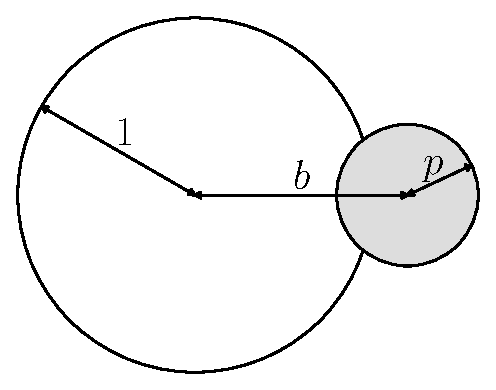
\includegraphics[width=\textwidth]{figures/geom.pdf}
    \end{center}
    \caption{Geometry of a transit. \figlabel{geom}}
\end{figure}



\end{document}
